\chapter{Tables and Figures}
\label{ch:tables-and-figures}

\begin{table}[H]
    \renewcommand{\arraystretch}{1.4}
    \begin{center}
        \begin{tabular}{ |p{0.3cm}| p{2.4cm}|p{2.4cm}|p{1.2cm}| p{1.7cm}|p{1cm}|p{1.7cm}|  }
            \hline
            \multicolumn{1}{| c}{}
            &\multicolumn{1}{| c}{\textbf{Group 1}}
            & \multicolumn{1}{| c}{\textbf{Group 2}}
            & \multicolumn{2}{| c |}{\textbf{Wilcoxon tests}}
            & \multicolumn{1}{c}{\textbf{r}}
            & \multicolumn{1}{| c |}{\textbf{padj}} \\
            & & & \textbf{z} & \textbf{p} & &         \\
            \hline
            \multirow{3}{*}{\textbf{E}}
            &Sophisticated &Contemporary &-4.2111 &p<0.01 &0.842 &p<0.01\\
            &Sophisticated &Unpretentious &-2.7188 &p<0.01 &0.544 &p<0.05\\
            &Contemporary &Unpretentious &3.8751 &p<0.01 &0.775 &p<0.01\\
            \hline
            \hline
            \multirow{2}{*}{\textbf{A}}
            &Sophisticated &Contemporary &4.2864 &p<0.01 &0.872 &p<0.01\\
            &Contemporary &Unpretentious &-4.2121 &p<0.01 &0.842 &p<0.01\\
            \hline
            \hline
            \multirow{2}{*}{\textbf{C}}
            &Sophisticated &Contemporary &3.0545 &p<0.01 &0.611 &p<0.01\\
            &Contemporary &Unpretentious &-2.7863 & p<0.01 & 0.546 &p<0.05\\
            \hline
            \hline
            \multirow{2}{*}{\textbf{N}}
            &Sophisticated &Contemporary &-3.9739 &p<0.01 & 0.797 &p<0.01\\
            &Contemporary &Unpretentious &3.7269 &p<0.01 &0.745 &p<0.01\\
            \hline
            \hline
            \multirow{3}{*}{\textbf{O}}
            &Sophisticated &Contemporary &4.2932 &p<0.01 & 0.859 &p<0.01\\
            &Sophisticated &Unpretentious &2.9869 &p<0.01 & 0.595 &p<0.01\\
            &Contemporary &Unpretentious &-3.9709 &p<0.01 & 0.794 &p<0.01\\
            \hline
        \end{tabular}
    \end{center}
    \captionsetup{width=13.5cm}
    \caption{The statistically significant comparisons in the first study of each group individually using the Wilcoxon
    signed-rank test and Bonferroni correction while measuring Five Personality Traits for Mascot-Speakers interaction.
    In addition reporting effect sizes which are large}
    \label{table:wilcoxMS1}
\end{table}


%%%%%%%%%%%%%%%%%%%%%%%%%%%%%%%%%%%%%%%%%%%%%%%%%%%%%%%%%%%%%%%%%%%%%%%%%%%%%%%%%%%%%%%%%%%%%%%%%%%%%%%%%%%%%%%%%%%%%%%%
\begin{table}
    \renewcommand{\arraystretch}{1}
    \begin{center}
        \begin{tabular}{ |p{2.5cm}| p{0.5cm}|p{0.5cm}|p{1.3cm}| p{1.7cm}|p{1cm}|p{1.7cm}|  }
            \hline
            \multicolumn{1}{| c}{}
            &\multicolumn{1}{| c}{\textbf{Group 1}}
            & \multicolumn{1}{| c}{\textbf{Group 2}}
            & \multicolumn{2}{| c |}{\textbf{Wilcoxon tests}}
            & \multicolumn{1}{c}{\textbf{r}}
            & \multicolumn{1}{| c |}{\textbf{padj}} \\
            & & & \textbf{z} & \textbf{p} & &         \\
            \hline
            \multirow{9}{*}{\textbf{Sophisticated}}
            &E &A &-3.9431 &p<0.01 &0.789 &p<0.01\\
            &E &N &3.6469 &p<0.01 &0.729 &p<0.01\\
            &E &O &-4.3459 &p<0.01 &0.869 &p<0.01\\
            &A &C &2.8937 & p<0.01 &0.579 &p<0.05\\
            &A &N &4.3732 &p<0.01 &0.875 &p<0.01\\
            &A &O &-3.3377 &p<0.01 &0.668 &p<0.01\\
            &C &N &4.1446 &p<0.01 &0.829 &p<0.01\\
            &C &O &-3.8436 &p<0.01 &0.762 &p<0.01\\
            &N &O &-4.373 &p<0.01 &0.875 &p<0.01\\
            \hline
            \hline
            \multirow{4}{*}{\textbf{Contemporary}}
            &E &A &4.2574 &p<0.01 &0.861 &p<0.01\\
            &E &C &4.2659 &p<0.01 &0.853 &p<0.01\\
            &E &N &4.1175 &p<0.01 &0.824 &p<0.01\\
            &E &O &4.2866 &p<0.01 &0.872 &p<0.01\\
            \hline
            \hline
            \multirow{7}{*}{\textbf{Unpretentious}}
            &E &A &-3.1034 &p<0.01 & 0.630 &p<0.05\\
            &E &N &4.3736 &p<0.01 & 0.875 &p<0.01\\
            &A &C &3.4615 &p<0.01 & 0.742 &p<0.01\\
            &A &N &4.3463 &p<0.01 & 0.869 &p<0.01\\
            &C &N &3.7949 &p<0.01 & 0.759 &p<0.01\\
            &C &O &-2.9387 &p<0.01 & 0.569 &p<0.05\\
            &N &O &-4.3734 &p<0.01 & 0.875 &p<0.01\\
            \hline
        \end{tabular}
    \end{center}
    \captionsetup{width=13.5cm}
    \caption{The statistically significant comparisons in the second study of each group individually using the Wilcoxon
    signed-rank test and Bonferroni correction while measuring Five Personality Traits for mascot-speakers interaction.
    In addition reporting effect sizes which are large.}
    \label{table:wilcoxMS2}
\end{table}
%%%%%%%%%%%%%%%%%%%%%%%%%%%%%%%%%%%%%%%%%%%%%%%%%%%%%%%%%%%%%%%%%%%%%%%%%%%%%%%%%%%%%%%%%%%%%%%%%%%%%%%%%%%%%%%%%%%%%%%%
\pagebreak
%%%%%%%%%%%%%%%%%%%%%%%%%%%%%%%%%%%%%%%%%%%%%%%%%%%%%%%%%%%%%%%%%%%%%%%%%%%%%%%%%%%%%%%%%%%%%%%%%%%%%%%%%%%%%%%%%%%%%%%%
\begin{table}
    \renewcommand{\arraystretch}{1}
    \begin{center}
        \begin{tabular} { |p{0.5cm}| p{2cm}|p{2cm}|p{1.5cm}| p{1.7cm}|p{1cm}|p{1.5cm}|  }
            \hline
            \multicolumn{1}{| c}{}
            &\multicolumn{1}{| c}{\textbf{Group 1}}
            & \multicolumn{1}{| c}{\textbf{Group 2}}
            & \multicolumn{2}{| c |}{\textbf{Wilcoxon tests}}
            & \multicolumn{1}{c}{\textbf{r}}
            & \multicolumn{1}{| c |}{\textbf{padj}} \\
            & & & \textbf{z} & \textbf{p} & &         \\
            \hline
            \multirow{6}{*}{\textbf{E}}
            &Yellow &Turquoise &3.5315 &p<0.01 &0.706 &p<0.01\\
            &Yellow &Blood-Red &4.185 &p<0.01 &0.837 &p<0.01\\
            &Yellow &Pink &3.8951 &p<0.01 &0.781 &p<0.01\\
            &Orange &Blood-Red &4.1461 &p<0.01 &0.829 &p<0.01\\
            &Turquoise &Blood-Red &3.3966 &p<0.01 &0.682 &p<0.01\\
            &Blood-Red &Pink &-3.5166 &p<0.01 &0.711 &p<0.01\\
            \hline
            \hline
            \multirow{6}{*}{\textbf{A}}
            &Yellow &Orange &3.6211 &p<0.01 &0.724 &p<0.01\\
            &Yellow &Blood-Red &4.0237 &p<0.01 &0.805 &p<0.01\\
            &Orange &Turquoise &-4.0613 &p<0.01 &0.832 &p<0.01\\
            &Orange &Pink &-4.294 &p<0.01 &0.859 &p<0.01\\
            &Turquoise &Blood-Red &4.2807 &p<0.01 &0.856 &p<0.01\\
            &Blood-Red &Pink &-4.1868 &p<0.01 &0.842 &p<0.01\\
            \hline
            \hline
            \multirow{6}{*}{\textbf{C}}
            &Yellow &Orange &3.3333 &p<0.01 &0.660 &p<0.01\\
            &Yellow &Blood-Red &3.1945 &p<0.01 &0.657 &p<0.05\\
            &Orange &Turquoise &-3.8186 &p<0.01 &0.767 &p<0.01\\
            &Orange &Pink &-3.7784 &p<0.01 &0.755 &p<0.01\\
            &Turquoise &Blood-Red &3.2405 &p<0.01 &0.644 &p<0.05\\
            &Blood-Red &Pink &-3.1456 &p<0.01 &0.619 &p<0.05\\
            \hline
            \hline
            \multirow{4}{*}{\textbf{N}}
            &Yellow &Blood-Red &-4.3193 &p<0.01 &0.864 &p<0.01\\
            &Orange &Blood-Red &-4.2602 &p<0.01 &0.862 &p<0.01\\
            &Turquoise &Blood-Red &-4.287 &p<0.01 &0.872 &p<0.01\\
            &Blood-Red &Pink &4.3738 &p<0.01 &0.875 &p<0.01\\
            \hline
            \hline
            \multirow{4}{*}{\textbf{O}}
            &Yellow &Blood-Red &3.4619 &p<0.01 &0.692 &p<0.01\\
            &Yellow &Pink &2.8482 &p<0.01 &0.574 &p<0.05\\
            &Orange &Blood-Red &3.0702 &p<0.01 &0.614 &p<0.05\\
            \hline
        \end{tabular}
    \end{center}
    \captionsetup{width=13.5cm}
    \caption{The statistically significant comparisons in the first study of each group individually using the Wilcoxon signed-rank
    test and Bonferroni correction while measuring Five Personality Traits for mascot-lamp interaction.
    In addition reporting effect sizes which are large.}
    \label{table:wilcoxML1}
\end{table}

\pagebreak
%%%%%%%%%%%%%%%%%%%%%%%%%%%%%%%%%%%%%%%%%%%%%%%%%%%%%%%%%%%%%%%%%%%%%%%%%%%%%%%%%%%%%%%%%%%%%%%%%%%%%%%%%%%%%%%%%%%%%%%%
\begin{table}
    \renewcommand{\arraystretch}{1}
    \begin{center}
        \begin{tabular}{ |p{1.9cm}| p{0.5cm}|p{0.5cm}|p{1.2cm}| p{1.9cm}|p{1cm}|p{1.5cm}|  }
            \hline
            \multicolumn{1}{| c}{}
            &\multicolumn{1}{| c}{\textbf{Group 1}}
            & \multicolumn{1}{| c}{\textbf{Group 2}}
            & \multicolumn{2}{| c |}{\textbf{Wilcoxon tests}}
            & \multicolumn{1}{c}{\textbf{r}}
            & \multicolumn{1}{| c |}{\textbf{padj}} \\
            & & & \textbf{z} & \textbf{p} & &         \\
            \hline
            \multirow{4}{*}{\textbf{Yellow}}
            &E &N &3.9296 &p<0.01 &0.789 &p<0.01\\
            &A &N &3.561 &p<0.01 &0.722 &p<0.01\\
            &C &N &3.4599 &p<0.01 &0.692 &p<0.01\\
            &N &O &-3.6295 &p<0.01 &0.721 &p<0.01\\
            \hline
            \hline
            \multirow{6}{*}{\textbf{Orange}}
            &E &A &4.0294 &p<0.01 &0.818 &p<0.01\\
            &E &C &0.679 &p<0.01 &0.679 &p<0.01\\
            &E &N &0.661 &p<0.01 &0.661 &p<0.01\\
            &A &O &-4.1086 &p<0.01 &0.840 &p<0.01\\
            &C &O &-2.9182 &p<0.01 &0.587 &p<0.05\\
            &N &O &-3.1376 &p<0.01 &0.636 &p<0.05\\
            \hline
            \hline
            \multirow{8}{*}{\textbf{Turquoise}}
            &E &A &-3.8621 &p<0.01 &0.776 &p<0.01\\
            &E &C &-3.339 &p<0.01 &0.668 &p<0.01\\
            &E &N &3.0291 &p<0.01 &0.617 &p<0.05\\
            &A &N &3.7697 &p<0.01 &0.754 &p<0.01\\
            &A &O &2.8456 &p<0.01 &0.552 &p<0.05\\
            &C &N &4.1879 &p<0.01 &0.843 &p<0.01\\
            &C &O &3.4339 &p<0.01 &0.687 &p<0.01\\
            &N &O &-3.4777 &p<0.01 &0.690 &p<0.01\\
            \hline
            \hline
            \multirow{7}{*}{\textbf{Blood Red}}
            &E &N &-4.3464 &p<0.01 &0.869 &p<0.01\\
            &E &O &-2.9088 &p<0.01 &0.596 &p<0.05\\
            &A &C &-2.9421 &p<0.01 &0.597 &p<0.05\\
            &A &N &-4.2335 &p<0.01 &0.857 &p<0.01\\
            &A &O &-3.2177 &p<0.01 &0.631 &p<0.05\\
            &C &N &-3.8625 &p<0.01 &0.773 &p<0.01\\
            &N &O &3.9709 &p<0.01 &0.794 &p<0.01\\
            \hline
            \hline
            \multirow{8}{*}{\textbf{Pink}}
            &E &A &-3.9842 &p<0.01 &0.797 &p<0.01\\
            &E &C &-3.4545 &p<0.01 &0.714 &p<0.01\\
            &E &N &3.6722 &p<0.01 &0.735 &p<0.01\\
            &A &N &4.2394 &p<0.01 &0.848 &p<0.01\\
            &A &O &3.9193 &p<0.01 &0.792 &p<0.01\\
            &C &N &4.2392 &p<0.01 &0.848 &p<0.01\\
            &C &O &3.1883 &p<0.01 &0.638 &p<0.05\\
            &N &O &-3.9322 &p<0.01 &0.794 &p<0.01\\
            \hline
        \end{tabular}
    \end{center}
    \captionsetup{width=13.5cm}
    \caption{The statistically significant comparisons in the second study of each group individually using the Wilcoxon signed-rank
    test and Bonferroni correction while measuring Five Personality Traits for mascot-lamp interaction.
    In addition reporting effect sizes which are large.}
    \label{table:wilcoxML2}
\end{table}
%%%%%%%%%%%%%%%%%%%%%%%%%%%%%%%%%%%%%%%%%%%%%%%%%%%%%%%%%%%%%%%%%%%%%%%%%%%%%%%%%%%%%%%%%%%%%%%%%%%%%%%%%%%%%%%%%%%%%%%%
\pagebreak
%%%%%%%%%%%%%%%%%%%%%%%%%%%%%%%%%%%%%%%%%%%%%%%%%%%%%%%%%%%%%%%%%%%%%%%%%%%%%%%%%%%%%%%%%%%%%%%%%%%%%%%%%%%%%%%%%%%%%%%%
\begin{table}
    \renewcommand{\arraystretch}{1.4}
    \begin{center}
        \begin{tabular}{ |p{0.5cm}| p{1.5cm}|p{1.5cm}|p{1.3cm}| p{1.6cm}|p{1cm}|p{1.5cm}|  }
            \hline
            \multicolumn{1}{| c}{}
            &\multicolumn{1}{| c}{\textbf{Group 1}}
            & \multicolumn{1}{| c}{\textbf{Group 2}}
            & \multicolumn{2}{| c |}{\textbf{Wilcoxon tests}}
            & \multicolumn{1}{c}{\textbf{r}}
            & \multicolumn{1}{| c |}{\textbf{padj}} \\
            & & & \textbf{z} & \textbf{p} & &         \\
            \hline
            \multirow{6}{*}{\textbf{E}}
            &Level-1 &Level-4 &-3.9316 &p<0.01 & 0.786 &p<0.01\\
            &Level-1 &Level-5 &-3.5756 &p<0.01 & 0.714 &p<0.01\\
            &Level-2 &Level-4 &-3.687 &p<0.01 &0.743 &p<0.01\\
            &Level-2 &Level-5 &-3.4301 &p<0.01 &0.678 &p<0.01\\
            &Level-3 &Level-4 &-3.545 &p<0.01 &0.708 &p<0.01\\
            &Level-3 &Level-5 &-2.9168 &p<0.01 & 0.582 &p<0.05\\
            \hline
            \hline
            \multirow{6}{*}{\textbf{A}}
            &Level-1 &Level-2 &-3.5566 &p<0.01 &0.703 &p<0.01\\
            &Level-1 &Level-3 &-3.6336 &p<0.01 &0.727 &p<0.01\\
            &Level-2 &Level-4 &3.028 &p<0.01 &0.595 &p<0.05\\
            &Level-2 &Level-5 &3.0421 &p<0.01 &0.608 &p<0.05\\
            &Level-3 &Level-4 &3.0827 &p<0.01 &0.617 &p<0.05\\
            &Level-3 &Level-5 &2.8476 &p<0.01 &0.552 &p<0.05\\
            \hline
            \hline
            \multirow{6}{*}{\textbf{C}}
            &Level-1 &Level-3 &-3.8995 &p<0.01 &0.809 &p<0.01\\
            &Level-1 &Level-4 &-4.0659 &p<0.01 &0.813 &p<0.01\\
            &Level-2 &Level-3 &-3.3019 &p<0.01 &0.657 &p<0.01\\
            &Level-2 &Level-4 &-3.817 &p<0.01 &0.767 &p<0.01\\
            &Level-3 &Level-5 &3.3624 &p<0.01 &0.671 &p<0.01\\
            &Level-4 &Level-5 &3.8499 &p<0.01 &0.784 &p<0.01\\
            \hline
            \hline
            \multirow{4}{*}{\textbf{N}}
            &Level-1 &Level-2 &3.326 &p<0.01 &0.665 &p<0.01\\
            &Level-1 &Level-3 &3.8172 &p<0.01 &0.779 &p<0.01\\
            &Level-1 &Level-4 &3.8607 &p<0.01 &0.776 &p<0.01\\
            &Level-1 &Level-5 &3.4724 &p<0.01 &0.694 &p<0.05\\
            \hline
            \hline
            \multirow{1}{*}{\textbf{O}}
            &Level-1 &Level-2 &-2.8243 &p<0.01 &0.578 &p<0.01\\
            \hline
        \end{tabular}
    \end{center}
    \captionsetup{width=13.5cm}
    \caption{The statistically significant comparisons in the first study of each group individually using the
    Wilcoxon signed-rank test and Bonferroni correction while measuring Five Personality
    Traits for mascot-mascot interaction.
    In addition reporting effect sizes which are large.}
    \label{table:wilcoxMM1}
\end{table}

\pagebreak
%%%%%%%%%%%%%%%%%%%%%%%%%%%%%%%%%%%%%%%%%%%%%%%%%%%%%%%%%%%%%%%%%%%%%%%%%%%%%%%%%%%%%%%%%%%%%%%%%%%%%%%%%%%%%%%%%%%%%%%%
\begin{table}
    \renewcommand{\arraystretch}{1.4}
    \begin{center}
        \begin{tabular}{ |p{1.3cm}| p{0.5cm}|p{0.5cm}|p{1.2cm}| p{1.7cm}|p{1cm}|p{1.5cm}|  }
            \hline
            \multicolumn{1}{| c}{}
            &\multicolumn{1}{| c}{\textbf{Group 1}}
            & \multicolumn{1}{| c}{\textbf{Group 2}}
            & \multicolumn{2}{| c |}{\textbf{Wilcoxon tests}}
            & \multicolumn{1}{c}{\textbf{r}}
            & \multicolumn{1}{| c |}{\textbf{padj}} \\
            & & & \textbf{z} & \textbf{p} & &         \\
            \hline
            \multirow{5}{*}{\textbf{Level-1}}
            &E &A &-2.9843 &p<0.01 &0.609 &p<0.05\\
            &E &N &-3.3934 &p<0.01 &0.671 &p<0.01\\
            &A &N &-3.0749 &p<0.01 &0.603 &p<0.05\\
            &C &N &-3.0975 &p<0.01 &0.620 &p<0.05\\
            &N &O &3.0542 &p<0.01 &0.604 &p<0.05\\
            \hline
            \hline
            \multirow{4}{*}{\textbf{Level-2}}
            &E &A &-3.7586 &p<0.01 &0.757 &p<0.01\\
            &A &C &3.1519 &p<0.01 &0.620 &p<0.05\\
            &A &N &3.3024 &p<0.01 &0.654 &p<0.01\\
            &A &O &3.1503 &p<0.01 &0.617 &p<0.05\\
            \hline
            \hline
            \multirow{7}{*}{\textbf{Level-3}}
            &E &A &-2.9298 &p<0.01 &0.584 &p<0.05\\
            &E &C &-3.3928 &p<0.01 &0.660 &p<0.01\\
            &A &N &3.8758 &p<0.01 &0.775 &p<0.01\\
            &A &O &3.303 &p<0.01 & 0.660 &p<0.01\\
            &C &N &4.039 &p<0.01 & 0.808 &p<0.01\\
            &C &O &3.6229 &p<0.01 & 0.722 &p<0.01\\
            &N &O &-3.1867 &p<0.01 &0.627 &p<0.05\\
            \hline
            \hline
            \multirow{6}{*}{\textbf{Level-4}}
            &E &A &3.5903 &p<0.01 &0.719 &p<0.01\\
            &E &N &4.1601 &p<0.01 &0.837 &p<0.01\\
            &E &O &3.8034 &p<0.01 &0.765 &p<0.01\\
            &A &C &-3.7747 &p<0.01 &0.759 &p<0.01\\
            &C &N &4.1315 &p<0.01 &0.826 &p<0.01\\
            &C &O &3.7164 &p<0.01 &0.738 &p<0.01\\
            \hline
            \hline
            \multirow{4}{*}{\textbf{Level-5}}
            &E &A &2.9346 &p<0.01 &0.587 &p<0.05\\
            &E &C &3.1512 &p<0.01 &0.617 &p<0.05\\
            &E &N &3.7113 &p<0.01 &0.748 &p<0.01\\
            &E &O &3.4195 &p<0.01 &0.684 &p<0.01\\
            \hline
        \end{tabular}
    \end{center}
    \captionsetup{width=13.5cm}
    \caption{The statistically significant comparisons in the second study of each group individually using the
    Wilcoxon signed-rank test and Bonferroni correction while measuring Five Personality
    Traits for mascot-mascot interaction.
    In addition reporting effect sizes which are large.}
    \label{table:wilcoxMM2}
\end{table}
%%%%%%%%%%%%%%%%%%%%%%%%%%%%%%%%%%%%%%%%%%%%%%%%%%%%%%%%%%%%%%%%%%%%%%%%%%%%%%%%%%%%%%%%%%%%%%%%%%%%%%%%%%%%%%%%%%%%%%%%
\pagebreak
%%%%%%%%%%%%%%%%%%%%%%%%%%%%%%%%%%%%%%%%%%%%%%%%%%%%%%%%%%%%%%%%%%%%%%%%%%%%%%%%%%%%%%%%%%%%%%%%%%%%%%%%%%%%%%%%%%%%%%%%
\begin{table}
    \renewcommand{\arraystretch}{1.4}
    \begin{center}
        \begin{tabular}{ |p{0.5cm}| p{1.9cm}|p{1.9cm}|p{1.2cm}| p{1.7cm}|p{1cm}|p{1.5cm}|  }
            \hline
            \multicolumn{1}{| c}{}
            &\multicolumn{1}{| c}{\textbf{Group 1}}
            & \multicolumn{1}{| c}{\textbf{Group 2}}
            & \multicolumn{2}{| c |}{\textbf{Wilcoxon tests}}
            & \multicolumn{1}{c}{\textbf{r}}
            & \multicolumn{1}{| c |}{\textbf{padj}} \\
            & & & \textbf{z} & \textbf{p} & &         \\
            \hline
            \multirow{4}{*}{\textbf{E}}
            &Yellow &Blood-Red &3.1011 &p<0.01 & 0.627 &p<0.05\\
            &Yellow &Pink &3.2335 &p<0.01 &0.650 &p<0.05\\
            &Orange &Blood-Red &3.7314 &p<0.01 & 0.751 &p<0.01\\
            &Orange &Pink &3.1295 &p<0.01 &0.627 &p<0.05\\
            \hline
            \hline
            \multirow{7}{*}{\textbf{A}}
            &Yellow &Turquoise &-3.8448 &p<0.01 &0.780 &p<0.01\\
            &Yellow &Blood-Red &3.7734 &p<0.01 &0.781 &p<0.01\\
            &Orange &Turquoise &-4.0936 &p<0.01 & 0.819 &p<0.01\\
            &Orange &Blood-Red &3.1542 &p<0.01 & 0.650 &p<0.05\\
            &Orange &Pink &-3.305 &p<0.01 &0.653 &p<0.01\\
            &Turquoise &Blood-Red &4.3755 &p<0.01 &0.875 &p<0.01\\
            &Blood-Red &Pink &-3.7573 &p<0.01 & 0.757 &p<0.01\\
            \hline
            \hline
            \multirow{5}{*}{\textbf{C}}
            &Yellow &Turquoise &-3.9161 &p<0.01 &0.791 &p<0.01\\
            &Orange &Turquoise &-3.204 &p<0.01 & 0.641 &p<0.05\\
            &Orange &Blood-Red &3.4736 &p<0.01 &0.697 &p<0.01\\
            &Turquoise &Blood-Red &4.0152 &p<0.01 & 0.802 &p<0.01\\
            &Turquoise &Pink &3.7126 &p<0.01 & 0.749 &p<0.01\\
            \hline
            \hline
            \multirow{4}{*}{\textbf{N}}
            &Yellow &Blood-Red &-3.8045 &p<0.01 &0.786 &p<0.01\\
            &Orange &Blood-Red &-3.5754 &p<0.01 &0.724 &p<0.01\\
            &Turquoise &Blood-Red &-4.1588 &p<0.01 &0.837 &p<0.01\\
            &Blood-Red &Pink &3.6195 &p<0.01 &0.724 &p<0.01\\

            \hline
            \hline
            \multirow{4}{*}{\textbf{O}}
            &Yellow &Orange &3.1986 &p<0.01 &0.658 &p<0.05\\
            &Yellow &Turquoise &3.461 &p<0.01 &0.704 &p<0.01\\
            &Yellow &Blood-Red &4.2273 &p<0.01 &0.845 &p<0.01\\
            &Yellow &Pink &4.2307 &p<0.01 &0.856 &p<0.01\\
            \hline
        \end{tabular}
    \end{center}
    \captionsetup{width=13.5cm}
    \caption{The statistically significant comparisons in the first study of each group individually using the Wilcoxon
    signed-rank test and Bonferroni correction while measuring Five Personality Traits for mascot-tablet interaction.
    In addition reporting effect sizes which are large.}
    \label{table:wilcoxMT1}
\end{table}

\pagebreak
%%%%%%%%%%%%%%%%%%%%%%%%%%%%%%%%%%%%%%%%%%%%%%%%%%%%%%%%%%%%%%%%%%%%%%%%%%%%%%%%%%%%%%%%%%%%%%%%%%%%%%%%%%%%%%%%%%%%%%%%
\begin{table}
    \renewcommand{\arraystretch}{1.4}
    \begin{center}
        \begin{tabular}{ |p{2cm}| p{0.5cm}|p{0.5cm}|p{1.3cm}| p{2.1cm}|p{1cm}|p{1.7cm}|  }
            \hline
            \multicolumn{1}{| c}{}
            &\multicolumn{1}{| c}{\textbf{Group 1}}
            & \multicolumn{1}{| c}{\textbf{Group 2}}
            & \multicolumn{2}{| c |}{\textbf{Wilcoxon tests}}
            & \multicolumn{1}{c}{\textbf{r}}
            & \multicolumn{1}{| c |}{\textbf{padj}} \\
            & & & \textbf{z} & \textbf{p} & &         \\
            \hline
            \multirow{5}{*}{\textbf{Yellow}}
            &E &C &2.9954 &p<0.01 &0.599 &p<0.05\\
            &E &N &3.4443 &p<0.01 &0.717 &p<0.01\\
            &E &O &-3.7585 &p<0.01 &0.751 &p<0.01\\
            &A &O &-3.8775 &p<0.01 &0.807 &p<0.01\\
            &C &O &-4.0453 &p<0.01 &0.810 &p<0.01\\
            &N &O &-4.1998 &p<0.01 &0.840 &p<0.01\\

            \hline
            \hline
            \multirow{3}{*}{\textbf{Orange}}
            &E &A &3.6158 &p<0.01 & 0.724 &p<0.01\\
            &E &N &3.0578 &p<0.01 &0.603 &p<0.05\\
            &A &C &-3.1027 &p<0.01 & 0.628 &p<0.05\\
            \hline
            \hline
            \multirow{7}{*}{\textbf{Turquoise}}
            &E &A &-3.7457 &p<0.01 &0.743 &p<0.01\\
            &E &C &-3.9292 &p<0.01 &0.787 &p<0.01\\
            &A &N &3.8643 &p<0.01 &0.773 &p<0.01\\
            &A &O &3.1941 &p<0.01 &0.639 &p<0.05\\
            &C &N &4.0721 &p<0.01 &0.826 &p<0.01\\
            &C &O &3.5643 &p<0.01 & 0.737 &p<0.01\\
            &N &O &-3.1846 &p<0.01 & 0.642 &p<0.05\\
            \hline
            \hline
            \multirow{5}{*}{\textbf{Blood-Red}}
            &E &N &-3.1303 &p<0.01 &0.622 &p<0.05\\
            &A &N &-3.6735 &p<0.01 &0.740 &p<0.01\\
            &A &O &-3.7897 &p<0.01 &0.774 &p<0.01\\
            &C &N &-3.0814 &p<0.01 &0.616 &p<0.05\\
            &N &O &3.3013 &p<0.01 &0.665 &p<0.01\\
            \hline
            \hline
            \multirow{4}{*}{\textbf{Pink}}
            &E &A &-3.1366 &p<0.01 &0.627 &p<0.01\\
            &A &N &3.2557 &p<0.01 &0.646 &p<0.01\\
            &A &O &2.9877 &p<0.01 &0.598 &p<0.05\\
            &C &N &2.8606 &p<0.01 & 0.582 &p<0.05\\
            \hline
        \end{tabular}
    \end{center}
    \captionsetup{width=13.5cm}
    \caption{The statistically significant comparisons in the second study of each group individually using the Wilcoxon
    signed-rank test and Bonferroni correction while measuring Five Personality Traits for mascot-tablet interaction.
    In addition reporting effect sizes which are large.}
    \label{table:wilcoxMT2}
\end{table}
%%%%%%%%%%%%%%%%%%%%%%%%%%%%%%%%%%%%%%%%%%%%%%%%%%%%%%%%%%%%%%%%%%%%%%%%%%%%%%%%%%%%%%%%%%%%%%%%%%%%%%%%%%%%%%%%%%%%%%%%
%%%%%%%%%%%%%%%%%%%%%%%%%%%%%%%%%%%%%%%%%%%%%%%%%%%%%%%%%%%%%%%%%%%%%%%%%%%%%%%%%%%%%%%%%%%%%%%%%%%%%%%%%%%%%%%%%%%%%%%%
%%%%%%%%%%%%%%%%%%%%%%%%%%%%%%%%%%%%%%%%%%%%%%%%%%%%%%%%%%%%%%%%%%%%%%%%%%%%%%%%%%%%%%%%%%%%%%%%%%%%%%%%%%%%%%%%%%%%%%%%
\chapter{Questionnaire for the user study}
\begin{figure}[hbt!]
    \centering
    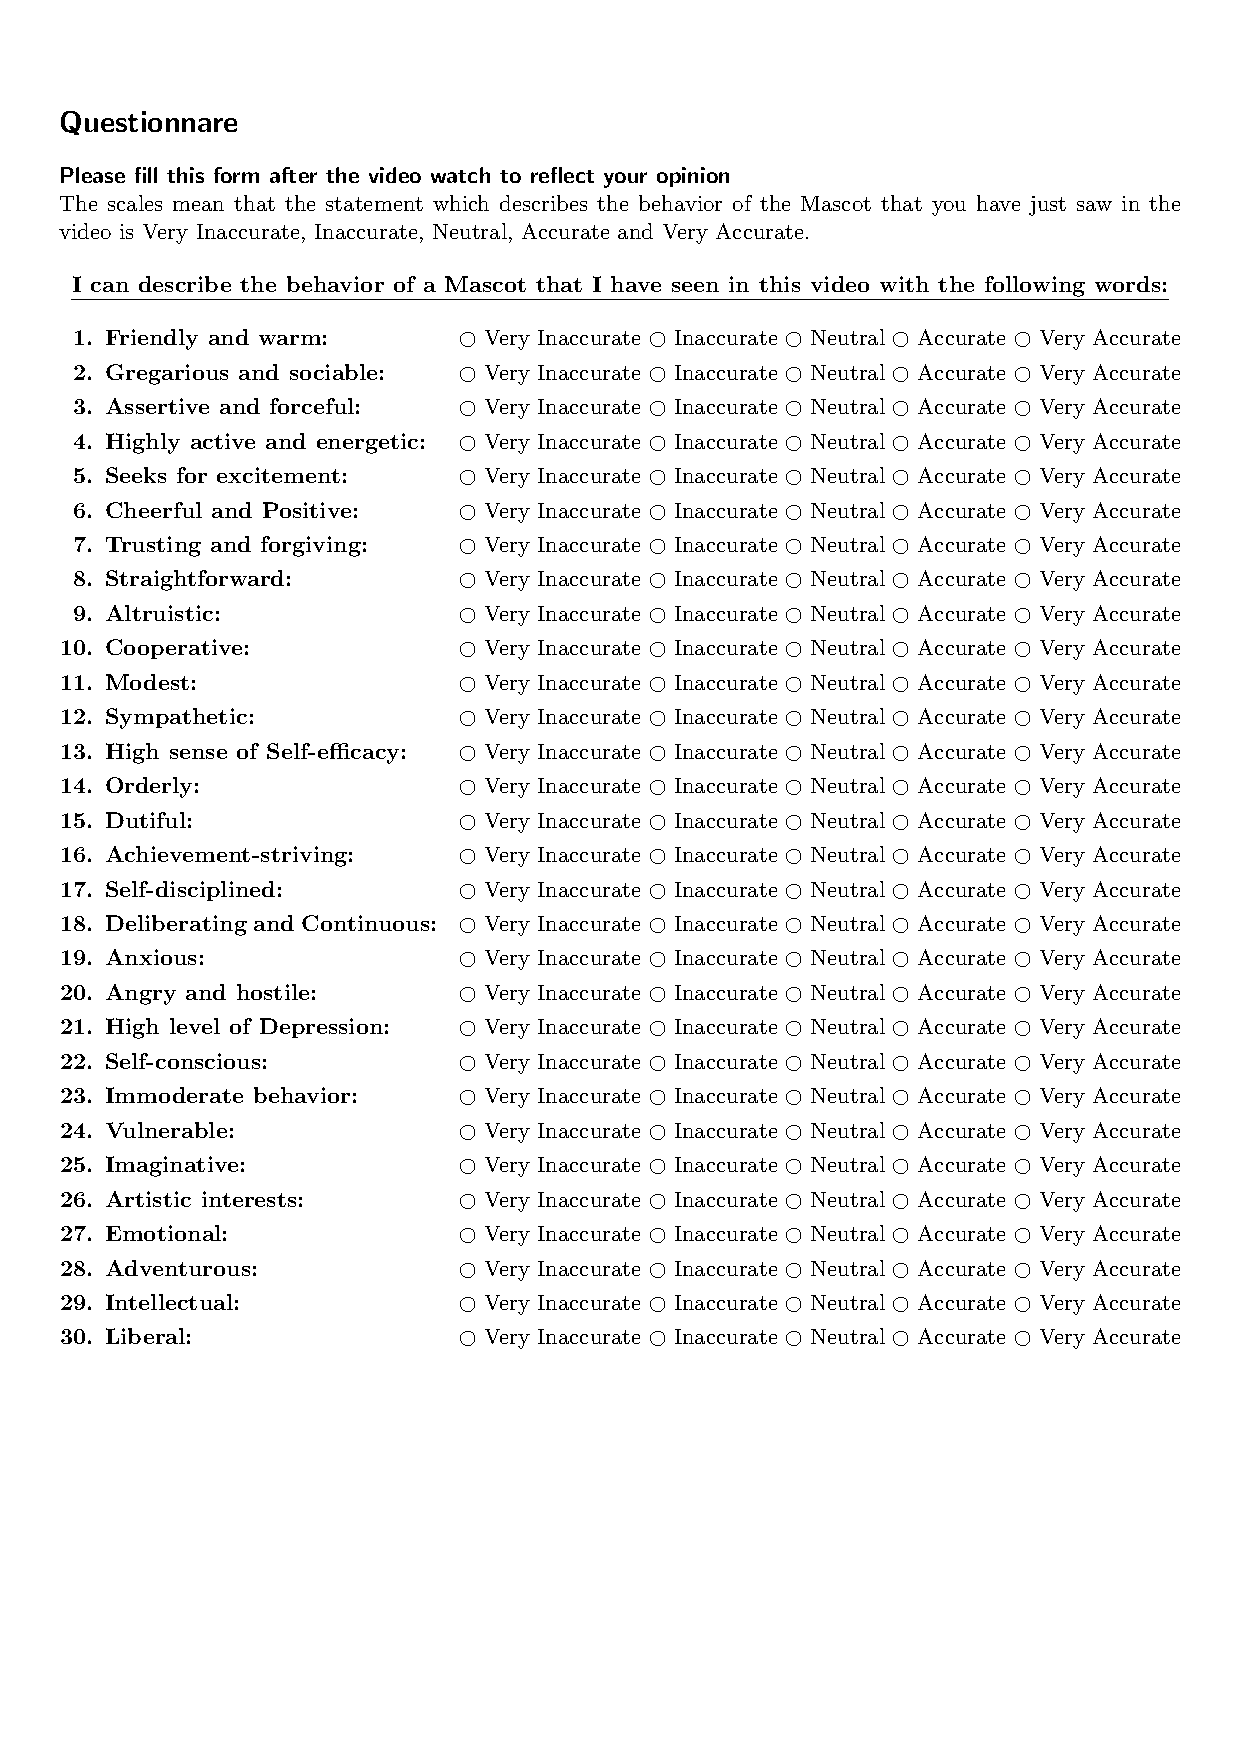
\includegraphics[scale=0.7]{Questionnare.pdf}
    \caption{The questionnaires given for each video during the experiments.}
    \label{fig:Questionnare}
\end{figure}
%%%%%%%%%%%%%%%%%%%%%%%%%%%%%%%%%%%%%%%%%%%%%%%%%%%%%%%%%%%%%%%%%%%%%%%%%%%%%%%%%%%%%%%%%%%%%%%%%%%%%%%%%%%%%%%%%%%%%%%%
%%%%%%%%%%%%%%%%%%%%%%%%%%%%%%%%%%%%%%%%%%%%%%%%%%%%%%%%%%%%%%%%%%%%%%%%%%%%%%%%%%%%%%%%%%%%%%%%%%%%%%%%%%%%%%%%%%%%%%%%
%
%\begin{table}[H]
%\renewcommand{\arraystretch}{1.7}
%\begin{center}
%\begin{tabular}{ |p{0.5cm}| p{2cm}|p{1.5cm}|p{1.5cm}| p{1.5cm}|p{1.5cm}|p{1.5cm}| p{1.5cm}| }
%\hline
%  \multicolumn{1}{| c}{}
%  & \multicolumn{1}{| c}{\textbf{Color}}
%  & \multicolumn{1}{| c}{\textbf{mean}}
%  & \multicolumn{1}{| c}{\textbf{min}}
%  & \multicolumn{1}{| c |}{\textbf{Q1}}
%  & \multicolumn{1}{c}{\textbf{median}}
%  & \multicolumn{1}{| c |}{\textbf{Q3}}
%  & \multicolumn{1}{c |}{\textbf{max}}\\
%\hline
%\multirow{5}{*}{\textbf{E}}
%&Yellow  &3.626667  &2.333333 &3.000000 &3.666667 &4.166667 &4.833333\\
%&Orange & 3.420000  &2.333333 &2.666667 &3.000000 &4.333333 &4.833333\\
%&Turquoise  &2.793333  &1.833333 &2.500000 &2.666667 &3.166667 &4.166667\\
%&Blood-Red  &2.006667  &1.000000 &1.500000 &1.666667 &2.500000 &4.500000\\
%&Pink  &2.760000  &1.666667 &2.166667 &2.833333 &3.166667 &3.666667\\
% \hline
% \hline
% \multirow{5}{*}{\textbf{A}}
%&Yellow  &3.380000  &1.833333 &2.333333 &3.666667 &4.000000 &5.000000\\
%&Orange  &2.286667  &1.000000 &1.833333 &2.333333 &2.666667 &3.333333\\
%&Turquoise  &3.453333  &2.000000 &2.833333 &3.500000 &3.833333 &5.000000\\
%&Blood-Red  &1.960000  &1.000000 &1.166667 &2.000000 &2.500000 &3.833333\\
%&Pink  &3.993333  &2.500000 &3.500000 &4.000000 &4.666667 &5.000000\\
% \hline
% \hline
% \multirow{5}{*}{\textbf{C}}
%&Yellow  &3.266667  &1.333333 &2.500000 &3.500000 &4.000000 &4.833333\\
%&Orange  &2.533333  &1.833333 &2.166667 &2.500000 &3.000000 &3.333333\\
%&Turquoise  &3.740000  &1.666667 &3.166667 &3.666667 &4.166667& 5.000000\\
%&Blood-Red  &2.493333  &1.166667 &1.500000 &2.166667 &3.500000 &4.666667\\
%&Pink  &3.546667 & 2.000000 &3.000000 &3.500000 &4.500000 &5.000000\\
% \hline
% \hline
% \multirow{5}{*}{\textbf{N}}
%&Yellow & 2.226667 & 1.000000 &1.500000 &2.166667 &3.000000 &3.333333\\
%&Orange & 2.313333 & 1.000000 &1.833333 &2.500000 &2.666667 &3.500000\\
%&Turquoise & 2.153333 & 1.000000 &1.333333 &2.000000 &3.000000 &3.500000\\
%&Blood-Red & 4.220000 & 3.166667 &3.833333 &4.333333 &4.500000 &5.000000\\
%&Pink & 1.880000 & 1.000000 &1.333333 &1.666667 &2.166667 &3.333333\\
% \hline
% \hline
% \multirow{5}{*}{\textbf{O}}
%&Yellow & 3.546667 & 1.500000 &3.000000 &3.500000 &4.166667 &5.000000\\
%&Orange & 3.080000 & 1.666667 &2.666667 &3.000000 &3.666667 &4.666667\\
%&Turquoise & 2.906667 & 2.333333 &2.500000 &2.833333 &3.333333 &3.666667\\
%&Blood-Red & 2.560000 & 1.166667 &1.833333 &2.666667 &3.166667 &4.000000\\
%&Pink & 2.826667 & 1.500000 &2.666667 &2.833333 &3.500000 &4.000000\\
% \hline
%\end{tabular}
%\end{center}
%\caption{Additional information to the Figure-1 for Mascot-Lamp use-case Study-1}
%\label{table:medianML1}
%\end{table}
%
%%%%%%%%%%%%%%%%%%%%%%%%%%%%%%%%%%%%%%%%%%%%%%%%%
%\begin{table}[H]
%\renewcommand{\arraystretch}{1.7}
%\begin{center}
%\begin{tabular}{ |p{2cm}| p{0.5cm}|p{1.5cm}|p{1.5cm}| p{1.5cm}|p{1.5cm}|p{1.5cm}| p{1.5cm}| }
%\hline
%  \multicolumn{1}{| c}{}
%  & \multicolumn{1}{| c}{\textbf{}}
%  & \multicolumn{1}{| c}{\textbf{mean}}
%  & \multicolumn{1}{| c}{\textbf{min}}
%  & \multicolumn{1}{| c |}{\textbf{Q1}}
%  & \multicolumn{1}{c}{\textbf{median}}
%  & \multicolumn{1}{| c |}{\textbf{Q3}}
%  & \multicolumn{1}{c |}{\textbf{max}}\\
%\hline
%\multirow{5}{*}{\textbf{Yellow}}
%&E &3.626667 & 2.333333 &3.000000 &3.666667 &4.166667 &4.833333\\
%&A &3.380000 & 1.833333 &2.333333 &3.666667 &4.000000 &5.000000\\
%&C &3.266667 & 1.333333 &2.500000 &3.500000 &4.000000 &4.833333\\
%&N &2.226667 & 1.000000 &1.500000 &2.166667 &3.000000 &3.333333\\
%&O &3.546667 & 1.500000 &3.000000 &3.500000 &4.166667 &5.000000\\
% \hline
% \hline
% \multirow{5}{*}{\textbf{Orange}}
%&E &3.420000 & 2.333333 &2.666667 &3.000000 &4.333333 &4.833333\\
%&A &2.286667 & 1.000000 &1.833333 &2.333333 &2.666667 &3.333333\\
%&C &2.533333 & 1.833333 &2.166667 &2.500000 &3.000000 &3.333333\\
%&N &2.313333 & 1.000000 &1.833333 &2.500000 &2.666667 &3.500000\\
%&O &3.080000 & 1.666667 &2.666667 &3.000000 &3.666667 &4.666667\\
% \hline
% \hline
% \multirow{5}{*}{\textbf{Turquoise}}
%&E & 2.793333 & 1.833333 &2.500000 &2.666667 &3.166667 &4.166667\\
%&A& 3.453333 & 2.000000 &2.833333 &3.500000 &3.833333 &5.000000\\
%&C &3.740000 & 1.666667 &3.166667 &3.666667 &4.166667 &5.000000\\
%&N &2.153333 & 1.000000 &1.333333 &2.000000 &3.000000 &3.500000\\
%&O &2.906667 & 2.333333 &2.500000 &2.833333 &3.333333 &3.666667\\
% \hline
% \hline
% \multirow{5}{*}{\textbf{Blood-Red}}
%&E &2.006667 & 1.000000 &1.500000 &1.666667 &2.500000 &4.500000\\
%&A &1.960000 & 1.000000 &1.166667 &2.000000 &2.500000 &3.833333\\
%&C &2.493333 & 1.166667 &1.500000 &2.166667 &3.500000 &4.666667\\
%&N &4.220000 & 3.166667 &3.833333 &4.333333 &4.500000 &5.000000\\
%&O &2.560000 & 1.166667 &1.833333 &2.666667 &3.166667 &4.000000\\
% \hline
% \hline
% \multirow{5}{*}{\textbf{Pink}}
%&E &2.760000 & 1.666667 &2.166667 &2.833333 &3.166667 &3.666667\\
%&A &3.993333 & 2.500000 &3.500000 &4.000000 &4.666667 &5.000000\\
%&C &3.546667 & 2.000000 &3.000000 &3.500000 &4.500000 &5.000000\\
%&N &1.880000 & 1.000000 &1.333333 &1.666667 &2.166667 &3.333333\\
%&O &2.826667 & 1.500000 &2.666667 &2.833333 &3.500000 &4.000000\\
% \hline
%\end{tabular}
%\end{center}
%\caption{Additional information to the Figure-2 for Mascot-Lamp use-case Study-2}
%\label{table:medianML2}
%\end{table}
%
%%%%%%%%%%%%%%%%%%%%%%%%%%%%%%%%%%%%%%%%%%%%%%%%%
%
%\begin{table}[H]
%\renewcommand{\arraystretch}{1.7}
%\begin{center}
%\begin{tabular}{ |p{0.5cm}| p{2cm}|p{1.5cm}|p{1.5cm}| p{1.5cm}|p{1.5cm}|p{1.5cm}| p{1.5cm}| }
%\hline
%  \multicolumn{1}{| c}{}
%  & \multicolumn{1}{| c}{\textbf{Genre Category}}
%  & \multicolumn{1}{| c}{\textbf{mean}}
%  & \multicolumn{1}{| c}{\textbf{min}}
%  & \multicolumn{1}{| c |}{\textbf{Q1}}
%  & \multicolumn{1}{c}{\textbf{median}}
%  & \multicolumn{1}{| c |}{\textbf{Q3}}
%  & \multicolumn{1}{c |}{\textbf{max}}\\
%\hline
%\multirow{3}{*}{\textbf{E}}
%&Sophisticated & 2.951111 & 1.388889 &2.666667 &3.055556 &3.333333 &3.833333\\
%&Contemporary & 4.080000 & 3.222222 &3.666667 &3.944444 &4.444444 &5.000000\\
%&Unpretentious & 3.231111 & 2.222222 &3.111111 &3.333333 &3.444444 &4.000000\\
% \hline
% \hline
% \multirow{3}{*}{\textbf{A}}
%&Sophisticated & 3.526667 & 2.944444 &3.222222 &3.333333 &3.722222 &4.666667\\
%&Contemporary & 2.704444 & 1.111111 &2.444444 &2.888889 &3.055556 &4.277778\\
%&Unpretentious & 3.700000 & 2.555556 &3.444444 &3.666667 &3.888889 &4.666667\\
% \hline
% \hline
% \multirow{3}{*}{\textbf{C}}
% &Sophisticated & 3.280000 & 2.444444 &3.000000 &3.166667 &3.500000 &4.611111\\
%&  Contemporary & 2.664444 & 1.000000 &2.111111 &2.777778 &3.166667 &4.055556\\
%& Unpretentious & 3.148889 & 1.888889 &3.000000 &3.166667 &3.444444 &4.666667\\
% \hline
% \hline
% \multirow{3}{*}{\textbf{N}}
%& Sophisticated & 2.328889 & 1.000000 &2.111111 &2.444444 &2.666667 &3.444444\\
%&  Contemporary & 3.188889 & 2.277778 &2.666667 &3.111111 &3.555556 &4.555556\\
%& Unpretentious & 2.335556 & 1.333333 &1.722222 &2.555556 &2.833333 &3.166667\\
% \hline
% \hline
% \multirow{3}{*}{\textbf{O}}
%& Sophisticated & 3.948889 & 3.111111 &3.611111 &3.833333 &4.222222 &4.944444\\
%&  Contemporary & 2.975556 & 2.000000 &2.722222 &2.944444 &3.222222 &4.000000\\
%& Unpretentious & 3.504444 & 2.555556 &3.166667 &3.388889 &3.833333 &4.666667\\
% \hline
%\end{tabular}
%\end{center}
%\caption{Additional information to the Figure-3 for Mascot-Speakers use-case Study-1}
%\end{table}
%
%%%%%%%%%%%%%%%%%%%%%%%%%%%%%%%%%%%%%%%%%%%%%%%%%
%\begin{table}[H]
%\renewcommand{\arraystretch}{1.7}
%\begin{center}
%\begin{tabular}{ |p{2.5cm}| p{0.5cm}|p{1.5cm}|p{1.5cm}| p{1.5cm}|p{1.5cm}|p{1.5cm}| p{1.5cm}| }
%\hline
%  \multicolumn{1}{| c}{}
%  & \multicolumn{1}{| c}{\textbf{}}
%  & \multicolumn{1}{| c}{\textbf{mean}}
%  & \multicolumn{1}{| c}{\textbf{min}}
%  & \multicolumn{1}{| c |}{\textbf{Q1}}
%  & \multicolumn{1}{c}{\textbf{median}}
%  & \multicolumn{1}{| c |}{\textbf{Q3}}
%  & \multicolumn{1}{c |}{\textbf{max}}\\
%\hline
%\multirow{3}{*}{\textbf{Sophisticated}}
%&E &2.951111 & 1.388889 &2.666667 &3.055556 &3.333333 &3.833333\\
%&A &3.526667 & 2.944444 &3.222222 &3.333333 &3.722222& 4.666667\\
%&C &3.280000 & 2.444444 &3.000000 &3.166667 &3.500000& 4.611111\\
%&N &2.328889 & 1.000000 &2.111111 &2.444444& 2.666667& 3.444444\\
%&O &3.948889 & 3.111111 &3.611111 &3.833333 &4.222222 &4.944444\\
% \hline
% \hline
% \multirow{3}{*}{\textbf{Contemporary}}
%&E &4.080000  &3.222222 &3.666667 &3.944444 &4.444444 &5.000000\\
%&A &2.704444  &1.111111& 2.444444 &2.888889 &3.055556 &4.277778\\
%&C &2.664444  &1.000000 &2.111111 &2.777778 &3.166667 &4.055556\\
%&N &3.188889  &2.277778 &2.666667& 3.111111 &3.555556 &4.555556\\
%&O &2.975556  &2.000000 &2.722222 &2.944444 &3.222222 &4.000000\\
% \hline
% \hline
% \multirow{3}{*}{\textbf{Unpretentious}}
%&      E& 3.231111 & 2.222222 &3.111111 &3.333333& 3.444444 &4.000000\\
%&     A & 3.700000 & 2.555556 &3.444444 &3.666667& 3.888889 &4.666667\\
%& C& 3.148889 & 1.888889 &3.000000 &3.166667 &3.444444 &4.666667\\
%&       N & 2.335556 & 1.333333 &1.722222 &2.555556& 2.833333 &3.166667\\
%&          O & 3.504444 & 2.555556 &3.166667 &3.388889 &3.833333 &4.666667\\
% \hline
%\end{tabular}
%\end{center}
%\caption{Additional information to the Figure-4 for Mascot-Speakers use-case Study-2}
%\end{table}
%
%%%%%%%%%%%%%%%%%%%%%%%%%%%%%%%%%%%%%%%%%%%%%%%%%
%\begin{table}[H]
%\renewcommand{\arraystretch}{1.7}
%\begin{center}
%\begin{tabular}{ |p{0.5cm}| p{2cm}|p{1.5cm}|p{1.5cm}| p{1.5cm}|p{1.5cm}|p{1.5cm}| p{1.5cm}| }
%\hline
%  \multicolumn{1}{| c}{}
%  & \multicolumn{1}{| c}{\textbf{Vibration}}
%  & \multicolumn{1}{| c}{\textbf{mean}}
%  & \multicolumn{1}{| c}{\textbf{min}}
%  & \multicolumn{1}{| c |}{\textbf{Q1}}
%  & \multicolumn{1}{c}{\textbf{median}}
%  & \multicolumn{1}{| c |}{\textbf{Q3}}
%  & \multicolumn{1}{c |}{\textbf{max}}\\
%\hline
%\multirow{5}{*}{\textbf{E}}
%&          Level1 & 2.166667 & 1.166667 &1.500000& 2.000000 &2.833333 &3.833333\\
%&          Level2 & 2.273333 & 1.166667 &1.500000 &2.000000 &3.000000 &4.000000\\
%&          Level3 & 2.586667 & 1.333333 &1.833333 &2.666667 &3.500000 &4.333333\\
%&          Level4 & 3.226667 & 2.166667& 2.500000 &3.000000 &3.666667 &4.666667\\
%&          Level5 & 3.773333 & 2.333333& 2.833333 &4.000000 &4.666667 &4.666667\\
% \hline
% \hline
% \multirow{5}{*}{\textbf{A}}
%&          Level1 & 2.573333 & 1.666667 &2.000000 &2.500000 &3.000000 &4.000000\\
%&          Level2 & 3.713333 & 2.000000 &3.166667 &4.000000 &4.333333 &4.666667\\
%&          Level3 & 3.800000 & 2.500000 &3.166667 &3.500000 &4.666667 &5.000000\\
%&          Level4 & 2.620000 & 1.333333 &1.833333 &2.833333 &3.166667 &4.000000\\
%&          Level5 & 2.546667 & 1.333333 &1.500000 &2.666667 &3.333333& 3.833333\\
% \hline
% \hline
% \multirow{5}{*}{\textbf{C}}
%&          Level1 & 2.606667 & 1.666667 &2.166667 &2.500000 &2.833333 &3.833333\\
%&          Level2 & 2.673333 & 1.500000 &2.000000& 2.666667 &3.500000 &4.166667\\
%&          Level3 & 3.960000 & 2.833333 &3.333333 &3.833333 &4.833333 &5.000000\\
%&          Level4 & 4.100000 & 2.166667 &3.666667 &4.000000 &4.666667 &5.000000\\
%&          Level5 & 2.740000 & 1.666667 &2.166667 &2.833333 &3.166667 &3.833333\\
% \hline
% \hline
% \multirow{5}{*}{\textbf{N}}
%&          Level1 & 3.606667 & 2.000000 &2.833333 &3.666667 &4.500000 &4.666667\\
%&          Level2 & 2.366667 & 1.333333 &1.666667 &2.166667 &3.166667 &3.666667\\
%&          Level3 & 2.186667 & 1.333333 &1.666667 &1.833333 &2.500000 &4.166667\\
%&          Level4 & 2.126667 & 1.000000 &1.666667 &2.166667 &2.500000 &3.500000\\
%&          Level5 & 2.266667 & 1.000000 &1.666667 &2.333333 &2.833333 &3.333333\\
% \hline
% \hline
% \multirow{5}{*}{\textbf{O}}
%&          Level1 & 2.420000 & 1.166667 &1.666667 &2.333333 &3.000000 &4.166667\\
%&          Level2 & 2.746667 & 1.833333 &2.166667 &2.500000 &3.166667 &4.500000\\
%&          Level3 & 3.186667 & 1.500000 &2.833333 &3.333333 &3.666667 &4.333333\\
%&          Level4 & 2.546667 & 1.000000 &1.666667 &2.666667 &3.333333 &4.500000\\
%&          Level5 & 2.560000 & 1.333333 &1.833333& 2.666667 &3.333333 &4.000000\\
% \hline
%\end{tabular}
%\end{center}
%\caption{Additional information to the Figure-5 for Mascot-Mascot use-case Study-1}
%\end{table}
%
%%%%%%%%%%%%%%%%%%%%%%%%%%%%%%%%%%%%%%%%%%%%%%%%%
%\begin{table}[H]
%\renewcommand{\arraystretch}{1.7}
%\begin{center}
%\begin{tabular}{ |p{2cm}| p{0.5cm}|p{1.5cm}|p{1.5cm}| p{1.5cm}|p{1.5cm}|p{1.5cm}| p{1.5cm}| }
%\hline
%  \multicolumn{1}{| c}{}
%  & \multicolumn{1}{| c}{\textbf{}}
%  & \multicolumn{1}{| c}{\textbf{mean}}
%  & \multicolumn{1}{| c}{\textbf{min}}
%  & \multicolumn{1}{| c |}{\textbf{Q1}}
%  & \multicolumn{1}{c}{\textbf{median}}
%  & \multicolumn{1}{| c |}{\textbf{Q3}}
%  & \multicolumn{1}{c |}{\textbf{max}}\\
%\hline
%\multirow{5}{*}{\textbf{Level1}}
%&      E & 2.166667 & 1.166667 &1.500000 &2.000000 &2.833333& 3.833333\\
%&     A & 2.573333 & 1.666667 &2.000000& 2.500000 &3.000000 &4.000000\\
%& C & 2.606667 & 1.666667& 2.166667 &2.500000 &2.833333 &3.833333\\
%&       N & 3.606667 & 2.000000 &2.833333 &3.666667 &4.500000 &4.666667\\
%&          O & 2.420000 & 1.166667 &1.666667 &2.333333 &3.000000 &4.166667\\
% \hline
% \hline
% \multirow{5}{*}{\textbf{Level2}}
%&      E & 2.273333 & 1.166667 &1.500000 &2.000000 &3.000000 &4.000000\\
%&     A & 3.713333 & 2.000000 &3.166667 &4.000000 &4.333333 &4.666667\\
%& C & 2.673333 & 1.500000 &2.000000 &2.666667 &3.500000 &4.166667\\
%&       N& 2.366667 & 1.333333 &1.666667 &2.166667& 3.166667 &3.666667\\
%&          O& 2.746667 & 1.833333 &2.166667 &2.500000 &3.166667 &4.500000\\
% \hline
% \hline
% \multirow{5}{*}{\textbf{Level3}}
%&      E & 2.586667 & 1.333333& 1.833333 &2.666667& 3.500000 &4.333333\\
%&     A& 3.800000 & 2.500000 &3.166667 &3.500000 &4.666667 &5.000000\\
%& C & 3.960000 & 2.833333 &3.333333 &3.833333 &4.833333 &5.000000\\
%&       N & 2.186667 & 1.333333 &1.666667 &1.833333 &2.500000 &4.166667\\
%&          O& 3.186667 & 1.500000 &2.833333 &3.333333 &3.666667 &4.333333\\
% \hline
% \hline
% \multirow{5}{*}{\textbf{Level4}}
%&      E & 3.226667 & 2.166667 &2.500000 &3.000000 &3.666667 &4.666667\\
%&     A & 2.620000 & 1.333333 &1.833333 &2.833333 &3.166667 &4.000000\\
%& C & 4.100000 & 2.166667 &3.666667 &4.000000& 4.666667 &5.000000\\
%&       N& 2.126667 & 1.000000 &1.666667 &2.166667 &2.500000 &3.500000\\
%&          O & 2.546667 & 1.000000 &1.666667& 2.666667 &3.333333 &4.500000\\
% \hline
% \hline
% \multirow{5}{*}{\textbf{Level5}}
%&      E & 3.773333 & 2.333333 &2.833333& 4.000000 &4.666667 &4.666667\\
%&     A & 2.546667 & 1.333333 &1.500000 &2.666667& 3.333333 &3.833333\\
%& C & 2.740000 & 1.666667 &2.166667 &2.833333& 3.166667 &3.833333\\
%&       N & 2.266667 & 1.000000 &1.666667 &2.333333 &2.833333& 3.333333\\
%&          O & 2.560000 & 1.333333 &1.833333 &2.666667 &3.333333 &4.000000\\
% \hline
%\end{tabular}
%\end{center}
%\caption{Additional information to the Figure-6 for Mascot-Mascot use-case Study-2}
%\end{table}
%
%%%%%%%%%%%%%%%%%%%%%%%%%%%%%%%%%%%%%%%%%%%%%%%%%
%\begin{table}[H]
%\renewcommand{\arraystretch}{1.7}
%\begin{center}
%\begin{tabular}{ |p{0.5cm}| p{2cm}|p{1.5cm}|p{1.5cm}| p{1.5cm}|p{1.5cm}|p{1.5cm}| p{1.5cm}| }
%\hline
%  \multicolumn{1}{| c}{}
%  & \multicolumn{1}{| c}{\textbf{Screen Color}}
%  & \multicolumn{1}{| c}{\textbf{mean}}
%  & \multicolumn{1}{| c}{\textbf{min}}
%  & \multicolumn{1}{| c |}{\textbf{Q1}}
%  & \multicolumn{1}{c}{\textbf{median}}
%  & \multicolumn{1}{| c |}{\textbf{Q3}}
%  & \multicolumn{1}{c |}{\textbf{max}}\\
%\hline
%\multirow{5}{*}{\textbf{E}}
%&    Yellow & 3.206667 & 2.000000 &3.000000 &3.333333 &3.666667& 4.000000\\
%&    Orange & 3.746667 & 1.666667 &2.833333 &4.166667 &4.666667 &5.000000\\
%& Turquoise & 2.873333 & 2.000000 &2.333333 &2.833333 &3.166667 &4.333333\\
%& Blood-Red & 2.253333 & 1.166667 &1.500000 &1.666667 &3.166667 &4.666667\\
%&      Pink & 2.626667 & 1.666667& 2.333333 &2.500000& 2.833333 &3.833333\\
% \hline
% \hline
% \multirow{5}{*}{\textbf{A}}
%&    Yellow & 2.773333 & 1.500000 &2.000000 &3.000000 &3.333333 &3.666667\\
%&    Orange & 2.440000 & 1.166667 &1.833333 &2.333333 &2.833333 &4.500000\\
%& Turquoise & 3.600000 & 1.833333 &3.333333 &3.666667 &4.000000 &4.166667\\
%& Blood-Red & 2.006667 & 1.000000 &1.500000 &1.833333 &2.500000 &3.333333\\
%&      Pink & 3.666667 & 1.666667 &3.000000 &3.666667& 4.666667 &5.000000\\
% \hline
% \hline
% \multirow{5}{*}{\textbf{C}}
%&    Yellow & 2.686667 & 1.833333 &2.333333 &2.666667 &3.000000 &3.500000\\
%&    Orange & 3.093333 & 2.166667 &2.500000 &2.666667 &3.833333 &4.500000\\
%& Turquoise & 3.986667 & 2.000000 &3.333333 &4.166667 &4.666667 &5.000000\\
%& Blood-Red & 2.360000 & 1.000000 &1.500000 &2.333333 &3.166667& 4.333333\\
%&      Pink & 2.960000 & 2.000000 &2.666667 &2.833333 &3.000000 &4.666667\\
% \hline
% \hline
% \multirow{5}{*}{\textbf{N}}
%&    Yellow & 2.373333 & 1.333333 &2.166667 &2.166667 &2.500000 &3.666667\\
%&    Orange & 2.560000 & 1.500000 &2.000000 &2.500000 &3.000000 &4.333333\\
%& Turquoise & 2.393333 & 1.000000 &2.000000 &2.500000 &2.666667 &3.500000\\
%& Blood-Red & 3.786667 & 1.500000 &3.000000 &3.833333 &4.666667 &5.000000\\
%&      Pink & 2.320000 & 1.166667 &1.833333 &2.333333 &2.500000 &4.166667\\
% \hline
% \hline
% \multirow{5}{*}{\textbf{O}}
%&    Yellow & 4.020000 & 2.500000 &3.500000 &4.000000 &4.666667 &5.000000\\
%&    Orange & 2.800000 & 1.333333 &1.833333 &3.000000 &3.500000 &5.000000\\
%& Turquoise & 3.053333 & 2.000000 &2.666667 &3.000000& 3.333333 &4.166667\\
%& Blood-Red & 2.586667 & 1.000000 &2.333333 &2.666667 &3.000000 &3.833333\\
%&      Pink & 2.726667 & 1.500000 &2.500000& 2.666667 &3.000000 &3.833333\\
% \hline
%\end{tabular}
%\end{center}
%\caption{Additional information to the Figure-7 for Mascot-Tablet use-case Study-1}
%\end{table}
%
%%%%%%%%%%%%%%%%%%%%%%%%%%%%%%%%%%%%%%%%%%%%%%%%%
%\begin{table}[H]
%\renewcommand{\arraystretch}{1.7}
%\begin{center}
%\begin{tabular}{ |p{2cm}| p{0.5cm}|p{1.5cm}|p{1.5cm}| p{1.5cm}|p{1.5cm}|p{1.5cm}| p{1.5cm}| }
%\hline
%  \multicolumn{1}{| c}{}
%  & \multicolumn{1}{| c}{\textbf{}}
%  & \multicolumn{1}{| c}{\textbf{mean}}
%  & \multicolumn{1}{| c}{\textbf{min}}
%  & \multicolumn{1}{| c |}{\textbf{Q1}}
%  & \multicolumn{1}{c}{\textbf{median}}
%  & \multicolumn{1}{| c |}{\textbf{Q3}}
%  & \multicolumn{1}{c |}{\textbf{max}}\\
%\hline
%\multirow{5}{*}{\textbf{Yellow}}
%&      E & 3.206667 & 2.000000 &3.000000& 3.333333& 3.666667& 4.000000\\
%&     A & 2.773333 & 1.500000 &2.000000 &3.000000 &3.333333& 3.666667\\
%& C & 2.686667 & 1.833333 &2.333333& 2.666667& 3.000000& 3.500000\\
%&       N & 2.373333 & 1.333333 &2.166667 &2.166667& 2.500000 &3.666667\\
%&          O & 4.020000 & 2.500000 &3.500000 &4.000000& 4.666667& 5.000000\\
% \hline
% \hline
% \multirow{5}{*}{\textbf{Orange}}
%&      E  &3.746667 & 1.666667& 2.833333 &4.166667 &4.666667& 5.000000\\
%&     A  &2.440000 & 1.166667 &1.833333 &2.333333 &2.833333 &4.500000\\
%& C &3.093333 & 2.166667 &2.500000 &2.666667 &3.833333 &4.500000\\
%&       N  &2.560000 & 1.500000 &2.000000 &2.500000& 3.000000 &4.333333\\
%&          O &2.800000 & 1.333333 &1.833333 &3.000000 &3.500000 &5.000000\\
% \hline
% \hline
% \multirow{5}{*}{\textbf{Turquoise}}
%&      E & 2.873333 & 2.000000 &2.333333 &2.833333 &3.166667 &4.333333\\
%&     A & 3.600000 & 1.833333 &3.333333 &3.666667 &4.000000 &4.166667\\
%& C & 3.986667 & 2.000000& 3.333333 &4.166667 &4.666667 &5.000000\\
%&       N & 2.393333 & 1.000000 &2.000000 &2.500000 &2.666667 &3.500000\\
%&          O & 3.053333 & 2.000000 &2.666667 &3.000000 &3.333333 &4.166667\\
% \hline
% \hline
% \multirow{5}{*}{\textbf{Blood-Red}}
%&      E & 2.253333 & 1.166667 &1.500000 &1.666667 &3.166667 &4.666667\\
%&     A & 2.006667 & 1.000000 &1.500000& 1.833333& 2.500000 &3.333333\\
%& C & 2.360000 & 1.000000 &1.500000 &2.333333& 3.166667 &4.333333\\
%&       N & 3.786667 & 1.500000 &3.000000& 3.833333 &4.666667 &5.000000\\
%&          O & 2.586667 & 1.000000 &2.333333 &2.666667 &3.000000 &3.833333\\
% \hline
% \hline
% \multirow{5}{*}{\textbf{Pink}}
%&      E & 2.626667 & 1.666667 &2.333333 &2.500000 &2.833333 &3.833333\\
%&     A & 3.666667 & 1.666667 &3.000000& 3.666667& 4.666667 &5.000000\\
%& C & 2.960000 & 2.000000 &2.666667 &2.833333 &3.000000 &4.666667\\
%&       N & 2.320000 & 1.166667 &1.833333 &2.333333 &2.500000 &4.166667\\
%&          O & 2.726667 & 1.500000 &2.500000 &2.666667 &3.000000 &3.833333\\
% \hline
%\end{tabular}
%\end{center}
%\caption{Additional information to the Figure-8 for Mascot-Tablet use-case Study-2}
%\end{table}
